\documentclass[../main.tex]{subfiles}

\begin{document}

\subsection{Alternative solutions and tradeoffs}

\begin{table}[H]
    \centering
    \caption{A comparison of the alternative solutions.}
    \label{tab:alt-solutions}
    \begin{tabular}{ p{4cm} p{6cm} p{6cm} }
        \toprule
        \textit{} & \textit{Design A} & \textit{Design B}\\ \midrule
        Type  & Custom made drone with onboard computer & Commercial drone with high performance and many features    \\
        Flexibility & Very flexible and and customization is easy & Hard to customize or modify it since it flies under limited protocols and standards. \\

        Price \& Availability & Cheaper but the shipping and building processes must be considered & Expensive but in our case its available in our hands and ready to fly.   \\

        Onboard computer & Must have & Must have \\
        \bottomrule
    \end{tabular}
\end{table} 

From the \cref{tab:alt-solutions} above, 
we can see some tradeoffs 
between design A and design B, but in both designs, 
an onboard microcomputer must be present for 
flying control and the support of autopilot feature. 
There are three options for onboard microcomputers, 
which are shown in the following 
\cref{tab:onboard-computers}. Raspberry Pi 4 seems 
to be the winner since it has advantages 
in specifications, connection interfaces, 
and availability.

\begin{table}[bt]
    \centering
    \caption{A comparison of the onboard computers.}
    \label{tab:onboard-computers}  
    \begin{tabular}{ p{3cm} p{4cm} p{4cm} p{4cm} }
        \toprule
        \textit{} & \textit{Raspberry Pi 4} & \textit{NVIDIA Jetson Nano} & \textit{\textsc{dji} Manifold}\\ \midrule
        Specifications  & CPU:Cortex-A72 (ARM v8) 64-bit@ 1.5GHz | Ram :4GB or 8GB LPDDR4-3200 SDRAM | GPU : Broadcom VideoCore VI & CPU:Quad-core ARM A57 @ 1.43 GHz | Ram: 4 GB 64-bit LPDDR4   | GPU:128-core Maxwell & CPU:Quad-core,ARM | Ram: 2 GB DDR3L | GPU:Low-power GeForce graphics processor \\ \addlinespace
        Connection interfaces & 2.4 GHz and 5.0 GHz IEEE 802.11ac wireless, Bluetooth 5.0 & Gigabit Ethernet \& M.2 Key E (for WiFi support). &10/100/1000 BASE-T Ethernet \\ \addlinespace

        Price \& Availability & 300 QAR available and can be used on any drone & 400 QAR available but need to be ordered and shipped & Very expensive and restricted to \textsc{dji} drones and \textsc{dji} company stopped selling it \\ \addlinespace
        Picture & \begin{minipage}{.2\textwidth}
            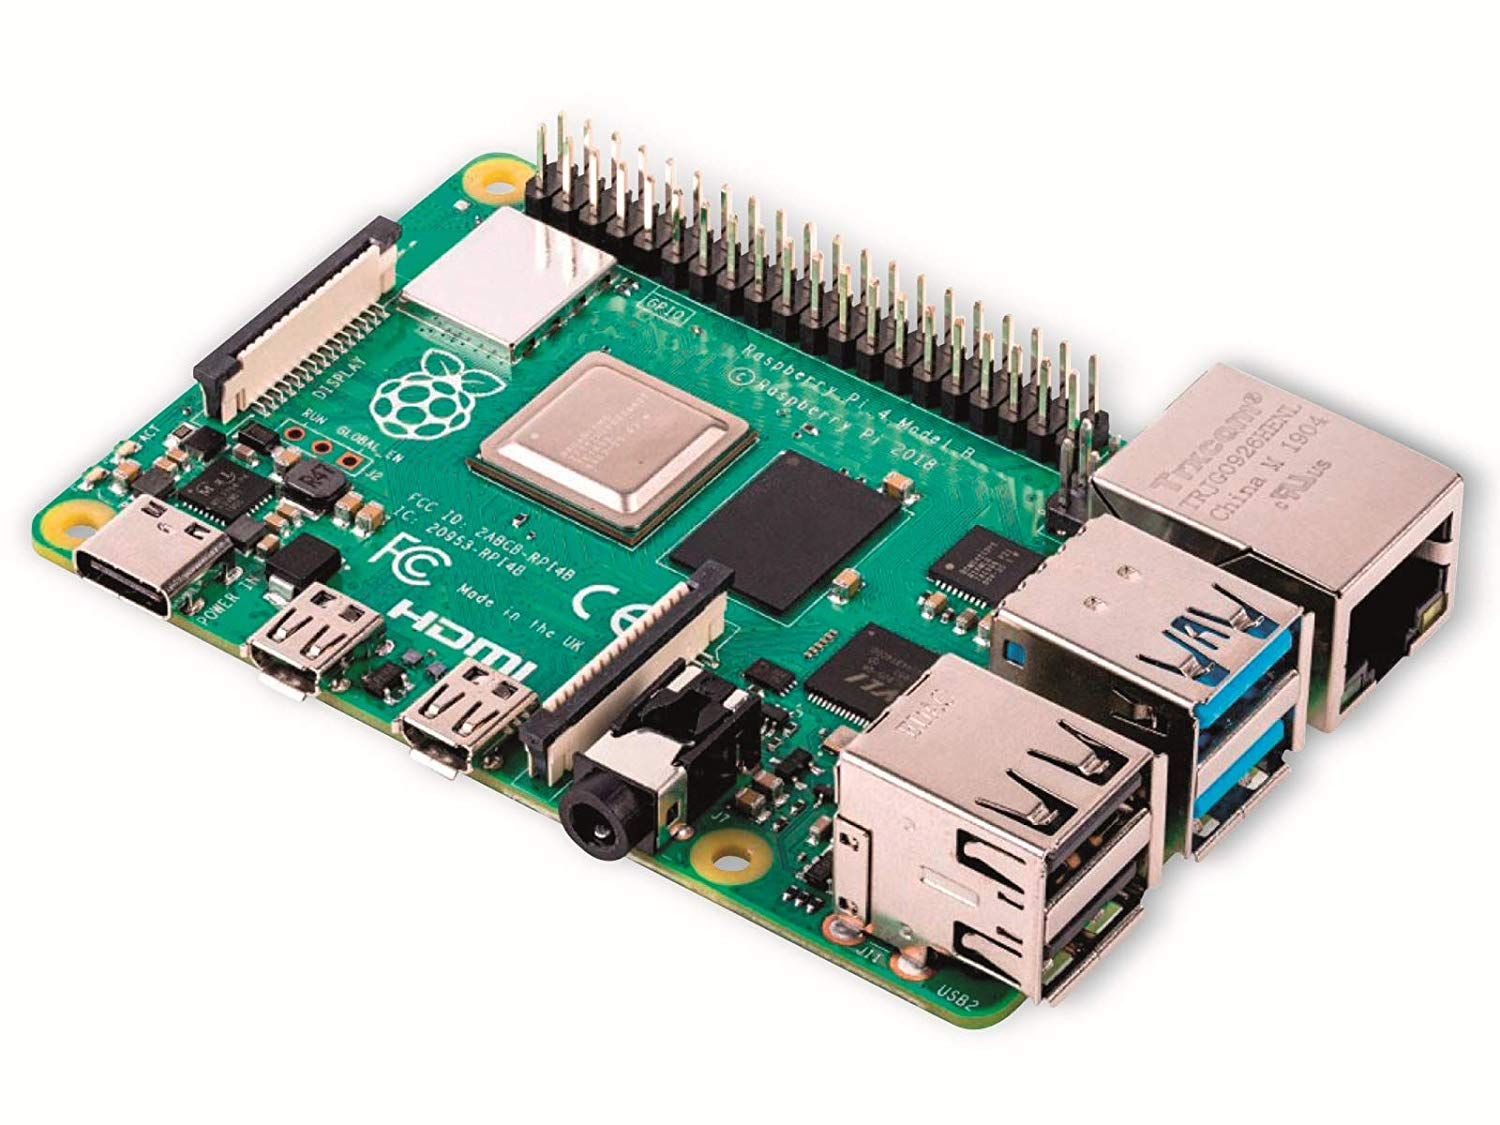
\includegraphics[width=40mm, height=30mm]{raspberry.jpg}
            \end{minipage}  & \begin{minipage}{.2\textwidth}
            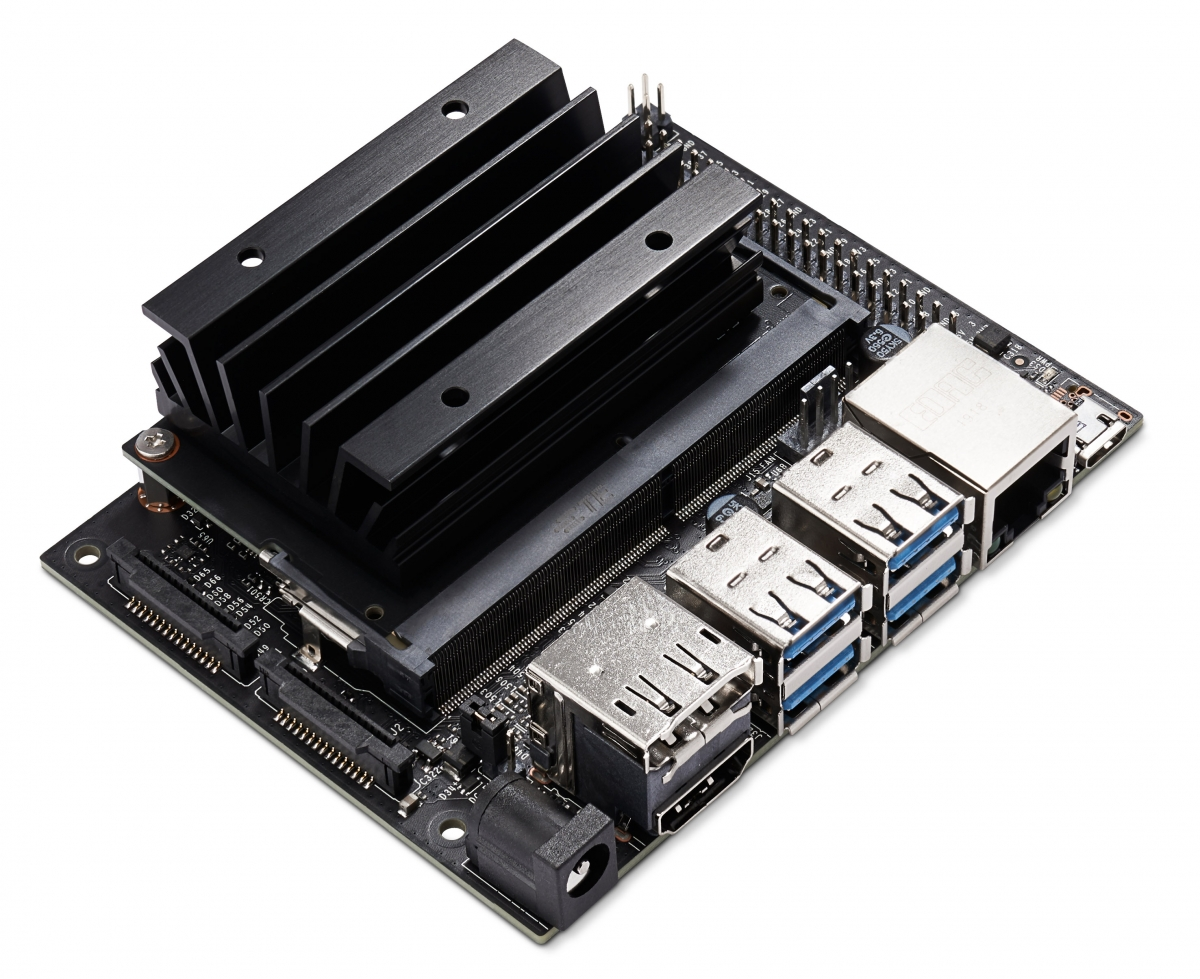
\includegraphics[width=40mm, height=30mm]{jetson.jpg}
            \end{minipage} & \begin{minipage}{.2\textwidth}
            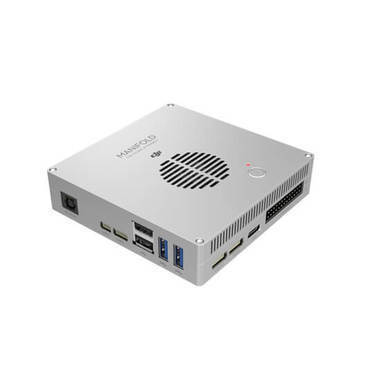
\includegraphics[width=40mm, height=30mm]{manifold.jpg}
        \end{minipage} \\
        \bottomrule
        \end{tabular}
    \end{table}

\subsection{Selected solution overview}\label{sec:selected-solution}

The proposed solution consists of two main parts: 
a commercial drone and a controlling system.
We have chosen the commercial drones especially 
the Parrot \textsc{anafi} for several reasons.
Firstly, it is supported by a continuously updated 
\textsc{sdk} and it can be controlled easily 
with a simple Python script which makes 
\gls{drl} development much easier and more stable. 

Secondly, it has a good flight time 
as the \textsc{anafi} drone has a 2700 mAh battery. 
It can fly up to 25 minutes which is good enough 
for our application.
Finally, its support of Wi-Fi 802.11 and \gls{gps} 
features is essential in our project for 
executing scripts and navigation. 

For how the system will work, firstly, the user 
will import or choose the mobility pattern and set
the constraints to the monitor device,
which is a laptop. Then, the laptop will send basic
high-level commands to the drone agent which is a
Raspberry Pi that in turn will apply certain
operations such as start and stop.

Once the user finishes importing the mobility pattern
and starting the drone mission, the drone will
take off and begin visiting areas and scanning for
the most number of mobile targets based on the
trained \gls{drl} model.
The user will keep receiving live updates and the
status of service on the control section using Wi-Fi.
Most of the connections in the system are wireless,
which will have benefits and drawbacks as discussed
in the \cref{sec:hardware-software} below.

\subsection{High level architecture}

\Cref{fig:arch-fig} shows a high-level architecture 
of the complete working system, in which a group 
of connected adapters and devices are combined into 
a single functional system. 
The architecture is composed of three sections namely
interfacing, controlling, and targets. 
The interfacing section contains the drone that 
will handle the onboard computer, its power source, 
and the connection adapters. 
In the controlling part, a personal computer 
will be responsible for contacting the onboard computer 
to adjust settings, execute scripts, and get 
live updates and results. 
Finally, there will be multiple moving targets 
in the target section. For example, 
R/C cars are controlled manually and moving in 
a specific mobility pattern with varying directions 
and destinations. 
In the next section, hardware and software components 
will be presented in a more detailed manner.

\begin{figure}[bt]
    \centering
    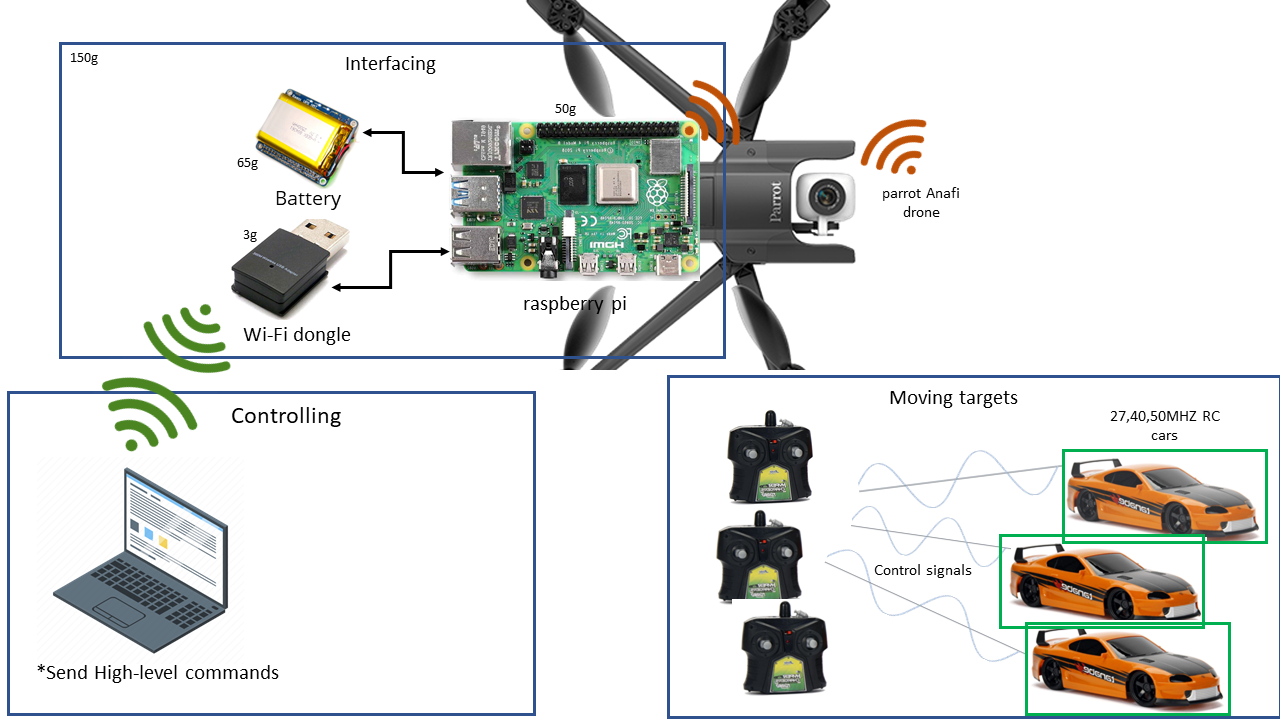
\includegraphics[width=0.9\textwidth]{high-level-arch.png}
    \caption{The high-level architecture of the overall system.}
    \label{fig:arch-fig}
\end{figure}


\subsection{Hardware/software to be used}\label{sec:hardware-software}

\subsubsection{Software}
    %parrot olympe
    %parrot sphinx
    %Gazebo simulator
    %roboflow
    %google colab notebook /jupyter notebook
There are three primary categories of software 
depending on the usage: simulation, training, 
and application. The first part will focus on 
simulating the environment, testing the models, 
and flight control. Before discussing the software 
to be used, we have selected Ubuntu 18.04 (Bionic Beaver) 
as an operating system for several reasons. 
One key reason is due to compatibility because 
Parrot's Olympe and Sphinx programs are only 
supported on limited distributions and operating systems,
one which is Ubuntu 18.04. 
Another reason is that it is a lite \textsc{os} 
and can be installed on the onboard computer that 
will be attached to the drone. For the simulation part, 
using Sphinx and Gazebo software is a very helpful tool 
to visualize the environment, control the drone, 
and apply the \gls{drl} model. Sphinx is a simulation 
tool built on top of Gazebo 
to run the Parrot's drone firmware on 
personal computers, which comes with helpful 
features for simulation like visualizing flight 
data at runtime, running the \gls{uav} remotely, 
and executing scripts with the command line. 
Gazebo is a robot \textsc{gui} simulation 
which simulates the visual and physical surrounding 
of drones and custom 3D objects. 
\Cref{fig:gazebo} shows how the Sphinx 
program looks like. 

\begin{figure}[bt]
    \centering
    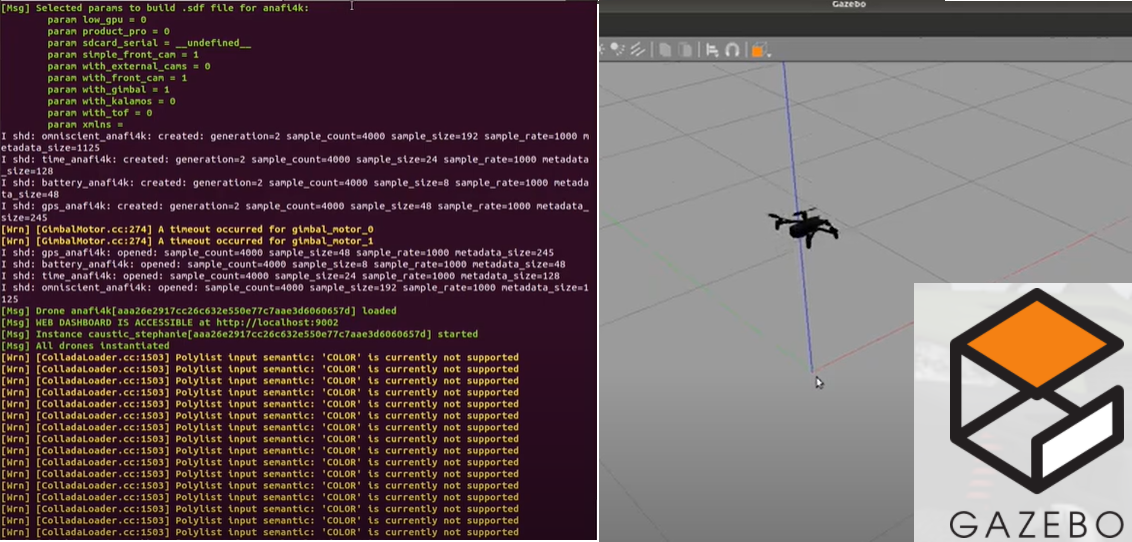
\includegraphics[width=0.9\textwidth]{gazebo.png}
    \caption{The Sphinx program that runs on top of Gazebo.}
    \label{fig:gazebo}
\end{figure}

In the training part, we used simulation tools to 
generate some training datasets. Firstly, 
we placed random objects and captured the images 
using the simulated drone camera. We have used a 
website called Roboflow which helped us labelling 
the objects and generate new datasets from the 
existing ones with different types of augmentation 
like rotation and scaling. 
For the object detection model, Google Colab notebook 
was a sufficient tool to start training using 
\gls{cnn} \textsc{yolo}v5 in addition to the 
Jupyter notebook which was very helpful 
in code experimentation. 

For the application software, Parrot Olympe 
was used to send commands to the physical as well as 
the simulated drone and control the flight trip and 
how the drone moves. Parrot Olympe uses Python 
controller programming interface for Parrot drones 
which makes controlling simple and easy using a 
Python script.

\subsubsection{Hardware}
    %Parrot ANAFI Drone
    %Raspberry Pi 4
    %lithium Battery
    %Wi-Fi adapter dongle
    %laptop control station
The main core of the hardware part is the drone, 
which will be the Parrot \textsc{anafi}. This model 
has a couple of features that made us choose it 
which have been listed in the 
\cref{sec:selected-solution} above. 
The second important device is the Raspberry Pi 
which will be used as an onboard computer and will 
handle several tasks such as:

\begin{enumerate}
    \item connecting to the drone 
        using a Wi-Fi interface,
    \item controlling the drone 
        by executing Olympe to send control signals 
        to and receive sensory data from the drone,
    \item applying the \gls{drl} model supported by 
        the command and control system,
    \item and receiving high-level commands and 
        sending data to the command and control system.
\end{enumerate}
 
The Parrot \textsc{anafi} is connected 
to the onboard computer using another 
2.4GHz Wi-Fi interface with the help of a 
300Mbps Wi-Fi adapter dongle connected to 
the Raspberry Pi through its \textsc{usb} interface. 
The power source for the Raspberry Pi will be a 
lithium battery with a power board called 
\textsc{UPSP}ack Standard Power Supply attached to 
the main Raspberry Pi board. It includes a 4000mAh 
lithium battery, which provides enough power 
and time for our application.
The connection between the Raspberry Pi and 
the power board is shown in \cref{fig:connection}.

\begin{figure}[bt]
    \centering
    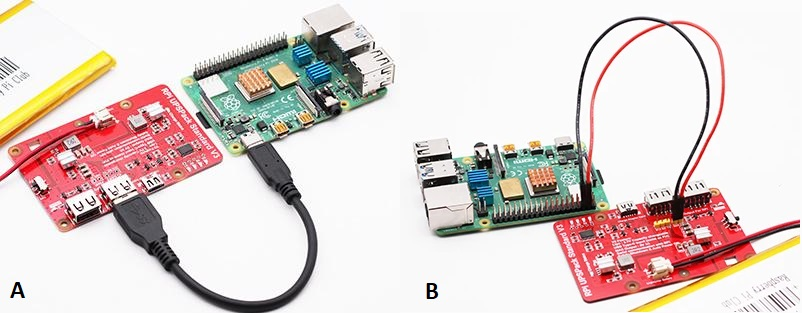
\includegraphics[width=0.6\textwidth]{connection.png}
    \caption{Raspberry Pi and power board connection.}
    \label{fig:connection}
\end{figure}     

\end{document}
